\documentclass[11pt,a4paper, english, swedish
]{article}
\pdfoutput=1

\usepackage{custom_as}

\graphicspath{ {figurer/} }

%%Drar in tabell och figurtexter
\usepackage[margin=10 pt]{caption}
%%För att lägga in 'att göra'-noteringar i texten
\usepackage{todonotes} %\todo{...}

%%För att själv bestämma marginalerna. 
\usepackage[
%            top    = 3cm,
%            bottom = 3cm,
%            left   = 3cm, right  = 3cm
]{geometry}

%%För att ändra hur rubrikerna ska formateras
%\renewcommand{\thesection}{...}


\newcommand{\PP}[1]{\ensuremath\mathcal{P}\left(#1\right)}


\begin{document}

\newgeometry{top=2cm}
%%%%%%%%%%%%%%%%% vvv Inbyggd titelsida vvv %%%%%%%%%%%%%%%%%

\title{ Behandling av experimentella resultat\\[2mm] 
\Large En introduktion för fysikstudenter om hur man ska hantera
mätresultat och feluppskattningar}
\author{Andréas Sundström\footnote{Synpunkter och förslag tas gärna
    emot till
\href{mailto:sundstrom.andreas@gmail.com}{\nolinkurl{sundstrom.andreas@gmail.com}}.}}
\date{\today, \quad\texttt{v\,0.0}}

\maketitle

%%%%%%%%%%%%%%%%% ^^^ Inbyggd titelsida ^^^ %%%%%%%%%%%%%%%%%

\subsection*{Förord}
\small
Det här kompendiet är skrivet som en introduktion till
feluppskattningar för det svenska IPhO-laget. Jag har försökt fatta
mig kort, men jag har en tendens att kunna dra iväg när jag
skriver. 

Det viktigaste innehållet finns i avsnitt~\ref{sec:feluppskattningar},
men jag tyckte att det behövs en liten teoretisk bakgrund också, den
finns i avsnitt~\ref{sec:statistik}. Det avsnittet ska man läsa om man
vill få en lite klarare bild om varför feluppskattningarna på det ena
eller andra viset. Sedan finns har jag även lagt till ett avsnitt om
approximationer. Detta avsnitt hör inte så mycket ihop med resten av
det här kompendiet, men det är matnyttigt att kunna göra
uppskattningar både för teoretiska och experimentella beräkningar. 
\begin{flushright}
Andréas Sunsdtröm\\ 
Göteborg, 2016-06-10
\end{flushright}
\normalsize

\tableofcontents
\clearpage
\restoregeometry

\addtocounter{section}{-1}
\section{Approximationer -- Taylorutvecklingar}

\begin{figure}
\centering
% GNUPLOT: LaTeX picture with Postscript
\begingroup
  \makeatletter
  \providecommand\color[2][]{%
    \GenericError{(gnuplot) \space\space\space\@spaces}{%
      Package color not loaded in conjunction with
      terminal option `colourtext'%
    }{See the gnuplot documentation for explanation.%
    }{Either use 'blacktext' in gnuplot or load the package
      color.sty in LaTeX.}%
    \renewcommand\color[2][]{}%
  }%
  \providecommand\includegraphics[2][]{%
    \GenericError{(gnuplot) \space\space\space\@spaces}{%
      Package graphicx or graphics not loaded%
    }{See the gnuplot documentation for explanation.%
    }{The gnuplot epslatex terminal needs graphicx.sty or graphics.sty.}%
    \renewcommand\includegraphics[2][]{}%
  }%
  \providecommand\rotatebox[2]{#2}%
  \@ifundefined{ifGPcolor}{%
    \newif\ifGPcolor
    \GPcolortrue
  }{}%
  \@ifundefined{ifGPblacktext}{%
    \newif\ifGPblacktext
    \GPblacktexttrue
  }{}%
  % define a \g@addto@macro without @ in the name:
  \let\gplgaddtomacro\g@addto@macro
  % define empty templates for all commands taking text:
  \gdef\gplbacktext{}%
  \gdef\gplfronttext{}%
  \makeatother
  \ifGPblacktext
    % no textcolor at all
    \def\colorrgb#1{}%
    \def\colorgray#1{}%
  \else
    % gray or color?
    \ifGPcolor
      \def\colorrgb#1{\color[rgb]{#1}}%
      \def\colorgray#1{\color[gray]{#1}}%
      \expandafter\def\csname LTw\endcsname{\color{white}}%
      \expandafter\def\csname LTb\endcsname{\color{black}}%
      \expandafter\def\csname LTa\endcsname{\color{black}}%
      \expandafter\def\csname LT0\endcsname{\color[rgb]{1,0,0}}%
      \expandafter\def\csname LT1\endcsname{\color[rgb]{0,1,0}}%
      \expandafter\def\csname LT2\endcsname{\color[rgb]{0,0,1}}%
      \expandafter\def\csname LT3\endcsname{\color[rgb]{1,0,1}}%
      \expandafter\def\csname LT4\endcsname{\color[rgb]{0,1,1}}%
      \expandafter\def\csname LT5\endcsname{\color[rgb]{1,1,0}}%
      \expandafter\def\csname LT6\endcsname{\color[rgb]{0,0,0}}%
      \expandafter\def\csname LT7\endcsname{\color[rgb]{1,0.3,0}}%
      \expandafter\def\csname LT8\endcsname{\color[rgb]{0.5,0.5,0.5}}%
    \else
      % gray
      \def\colorrgb#1{\color{black}}%
      \def\colorgray#1{\color[gray]{#1}}%
      \expandafter\def\csname LTw\endcsname{\color{white}}%
      \expandafter\def\csname LTb\endcsname{\color{black}}%
      \expandafter\def\csname LTa\endcsname{\color{black}}%
      \expandafter\def\csname LT0\endcsname{\color{black}}%
      \expandafter\def\csname LT1\endcsname{\color{black}}%
      \expandafter\def\csname LT2\endcsname{\color{black}}%
      \expandafter\def\csname LT3\endcsname{\color{black}}%
      \expandafter\def\csname LT4\endcsname{\color{black}}%
      \expandafter\def\csname LT5\endcsname{\color{black}}%
      \expandafter\def\csname LT6\endcsname{\color{black}}%
      \expandafter\def\csname LT7\endcsname{\color{black}}%
      \expandafter\def\csname LT8\endcsname{\color{black}}%
    \fi
  \fi
  \setlength{\unitlength}{0.0500bp}%
  \begin{picture}(6802.00,3968.00)%
    \gplgaddtomacro\gplbacktext{%
      \csname LTb\endcsname%
      \put(462,704){\makebox(0,0)[r]{\strut{}-2}}%
      \csname LTb\endcsname%
      \put(462,1316){\makebox(0,0)[r]{\strut{}-1}}%
      \csname LTb\endcsname%
      \put(462,1929){\makebox(0,0)[r]{\strut{} 0}}%
      \csname LTb\endcsname%
      \put(462,2541){\makebox(0,0)[r]{\strut{} 1}}%
      \csname LTb\endcsname%
      \put(462,3153){\makebox(0,0)[r]{\strut{} 2}}%
      \csname LTb\endcsname%
      \put(594,484){\makebox(0,0){\strut{}-4}}%
      \csname LTb\endcsname%
      \put(1320,484){\makebox(0,0){\strut{}-3}}%
      \csname LTb\endcsname%
      \put(2047,484){\makebox(0,0){\strut{}-2}}%
      \csname LTb\endcsname%
      \put(2773,484){\makebox(0,0){\strut{}-1}}%
      \csname LTb\endcsname%
      \put(3500,484){\makebox(0,0){\strut{} 0}}%
      \csname LTb\endcsname%
      \put(4226,484){\makebox(0,0){\strut{} 1}}%
      \csname LTb\endcsname%
      \put(4952,484){\makebox(0,0){\strut{} 2}}%
      \csname LTb\endcsname%
      \put(5679,484){\makebox(0,0){\strut{} 3}}%
      \csname LTb\endcsname%
      \put(6405,484){\makebox(0,0){\strut{} 4}}%
      \put(3499,154){\makebox(0,0){\strut{}\Large$x$}}%
    }%
    \gplgaddtomacro\gplfronttext{%
      \csname LTb\endcsname%
      \put(2908,3740){\makebox(0,0)[r]{\strut{}$\sin(x)$}}%
      \csname LTb\endcsname%
      \put(2908,3520){\makebox(0,0)[r]{\strut{}$x$}}%
      \csname LTb\endcsname%
      \put(5083,3740){\makebox(0,0)[r]{\strut{}$x - \nicefrac{x^3}{6}$}}%
      \csname LTb\endcsname%
      \put(5083,3520){\makebox(0,0)[r]{\strut{}$x - \nicefrac{x^3}{6} + \nicefrac{x^5}{120}$}}%
    }%
    \gplbacktext
    \put(0,0){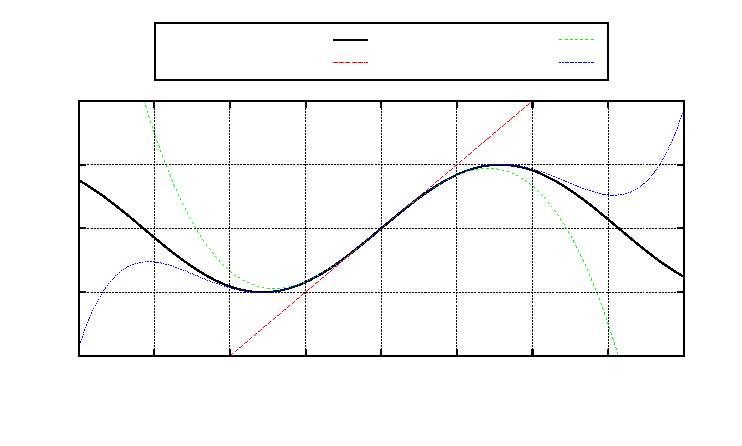
\includegraphics{taylor_sin}}%
    \gplfronttext
  \end{picture}%
\endgroup

\caption{}
\label{fig_taylor_sin}
\end{figure}



\section{Sannolihetslära och statistik}\label{sec:statistik}
När man gör mätningar vill man oftast ta reda på någon storhets värde
-- exempelvis periodtiden på en pendel. Med en mätning kan man dock
inte säga något om hur bra mätningen var. Men med flera mätningar kan
vi börja göra statistik över dem. Då 

Jag vill även betona vikten av statistik i framtida vetenskapliga och
tekniska karriärer. \emph{Statistik är ett mycket kraftfullt verktyg.}
Statistiken, när man börjar behärska den, är mycket mer än bara
''medelvärden och standardavvikelser''; den spelar en väsentlig roll i
mer eller mindre all experimentell vetenskap -- särskilt vid
feluppskattningar. 

\subsection{Stokastiska variabler}

\subsection{Sannolikhetsfördelningar och täthetsfunktioner}
Den statistik och sannolikhetslära man får lära sig i gymnasiet brukar
fördet mesta vara diskret (och ändlig). Alltså att det finns ett
ändligt antal möjliga utfall och varje utfall är distikt. Exempel på
detta är tärningskast, lottdragning och kortlekar. 

Verkligheten är dock oftast mer komplicerad än så. När man gör
mätningar handrar det oftas om mätnigar av en reellvärd
storhet som t.ex. en längd\footnotemark{}. Detta betyder att längden
kommer att anta ett reellt antal milimetrar och inte vara begränsad
till ett ändligt antal möjliga värden. För att analysera detta behövs
statistik för kontinuerliga fördelningar. 
\footnotetext{''Aha!'' tänker ni: atomer och kvantfysik gör att det
  bara finns diskreta längder. ''Nähä!'' säger jag: som fysiker måste
  man kunna hantera approximationer och veta begränsningarna i sina
  mätningar. Med en linjal eller skujtmått finns det ingen chans i
  världen att man skulle kunna stöta på problem orsakade av
  kvantfysik. Man kan alltså betrakta det som om de möjliga värden
  som längden kan anta ligger kontinuerligt.}

Sannolikhetsfördelningar karakteriseras av sin täthetsfunktion, som
brukar betecknas~$f$. Täthetsfunktionen talar om hur sannolikt det är
att få ett värde i ett visst intervall. Notera dock att den
\emph{inte} ger sannolikheten att få ett specifikt värde. Eftersom
det finns (ouppräknerligt) oändligt många möjliga utfall så är
sannolikheten att få ett visst exat värde
\begin{equation}
\PP{X=x}\; \text{''=''}\; \frac{1}{\infty}\; \text{''=''}\;0.
\end{equation}

För att beräkna sannolikheten att få sitt utfall $X$ i ett visst
intervall $[a, b]$ måste man integrera:
\begin{equation}
\PP{a<X<b} = \int_a^b f(x) \id{x}.
\end{equation}
Sannolikheten att få $a<X<b$ bestäms av täthetsfunktionen och
intevallet och motsvarar arean under $f(x)$.



\subsubsection{Normalfördelningen}
En av de vanligaste fördelningarna är normalfördelningen. Den
har täthesfunktionen
\begin{equation}
f(x) = \frac{1}{\sqrt{2\pi\sigma^2}} \, \ee^{-\frac{(x-\mu)^2}{2\sigma^2}},
\end{equation}
där $\mu$ är fördelningens \emph{väntevärde} och $\sigma$ är dess
\emph{standardavvikelse}. I \figref{fig:normal_dist} visas
täthetsfunktionen för några olika val av $\mu$ och $\sigma$. Där ser
vi att $\mu$ svarar mot var någonstans fördelnigen är centrerad, och
att $\sigma$ svarar mot hur bred fördelningen blir. 

\begin{figure}
\centering
% GNUPLOT: LaTeX picture with Postscript
\begingroup
  \makeatletter
  \providecommand\color[2][]{%
    \GenericError{(gnuplot) \space\space\space\@spaces}{%
      Package color not loaded in conjunction with
      terminal option `colourtext'%
    }{See the gnuplot documentation for explanation.%
    }{Either use 'blacktext' in gnuplot or load the package
      color.sty in LaTeX.}%
    \renewcommand\color[2][]{}%
  }%
  \providecommand\includegraphics[2][]{%
    \GenericError{(gnuplot) \space\space\space\@spaces}{%
      Package graphicx or graphics not loaded%
    }{See the gnuplot documentation for explanation.%
    }{The gnuplot epslatex terminal needs graphicx.sty or graphics.sty.}%
    \renewcommand\includegraphics[2][]{}%
  }%
  \providecommand\rotatebox[2]{#2}%
  \@ifundefined{ifGPcolor}{%
    \newif\ifGPcolor
    \GPcolortrue
  }{}%
  \@ifundefined{ifGPblacktext}{%
    \newif\ifGPblacktext
    \GPblacktexttrue
  }{}%
  % define a \g@addto@macro without @ in the name:
  \let\gplgaddtomacro\g@addto@macro
  % define empty templates for all commands taking text:
  \gdef\gplbacktext{}%
  \gdef\gplfronttext{}%
  \makeatother
  \ifGPblacktext
    % no textcolor at all
    \def\colorrgb#1{}%
    \def\colorgray#1{}%
  \else
    % gray or color?
    \ifGPcolor
      \def\colorrgb#1{\color[rgb]{#1}}%
      \def\colorgray#1{\color[gray]{#1}}%
      \expandafter\def\csname LTw\endcsname{\color{white}}%
      \expandafter\def\csname LTb\endcsname{\color{black}}%
      \expandafter\def\csname LTa\endcsname{\color{black}}%
      \expandafter\def\csname LT0\endcsname{\color[rgb]{1,0,0}}%
      \expandafter\def\csname LT1\endcsname{\color[rgb]{0,1,0}}%
      \expandafter\def\csname LT2\endcsname{\color[rgb]{0,0,1}}%
      \expandafter\def\csname LT3\endcsname{\color[rgb]{1,0,1}}%
      \expandafter\def\csname LT4\endcsname{\color[rgb]{0,1,1}}%
      \expandafter\def\csname LT5\endcsname{\color[rgb]{1,1,0}}%
      \expandafter\def\csname LT6\endcsname{\color[rgb]{0,0,0}}%
      \expandafter\def\csname LT7\endcsname{\color[rgb]{1,0.3,0}}%
      \expandafter\def\csname LT8\endcsname{\color[rgb]{0.5,0.5,0.5}}%
    \else
      % gray
      \def\colorrgb#1{\color{black}}%
      \def\colorgray#1{\color[gray]{#1}}%
      \expandafter\def\csname LTw\endcsname{\color{white}}%
      \expandafter\def\csname LTb\endcsname{\color{black}}%
      \expandafter\def\csname LTa\endcsname{\color{black}}%
      \expandafter\def\csname LT0\endcsname{\color{black}}%
      \expandafter\def\csname LT1\endcsname{\color{black}}%
      \expandafter\def\csname LT2\endcsname{\color{black}}%
      \expandafter\def\csname LT3\endcsname{\color{black}}%
      \expandafter\def\csname LT4\endcsname{\color{black}}%
      \expandafter\def\csname LT5\endcsname{\color{black}}%
      \expandafter\def\csname LT6\endcsname{\color{black}}%
      \expandafter\def\csname LT7\endcsname{\color{black}}%
      \expandafter\def\csname LT8\endcsname{\color{black}}%
    \fi
  \fi
  \setlength{\unitlength}{0.0500bp}%
  \begin{picture}(6802.00,3968.00)%
    \gplgaddtomacro\gplbacktext{%
      \csname LTb\endcsname%
      \put(946,704){\makebox(0,0)[r]{\strut{} 0}}%
      \csname LTb\endcsname%
      \put(946,1454){\makebox(0,0)[r]{\strut{} 0.1}}%
      \csname LTb\endcsname%
      \put(946,2204){\makebox(0,0)[r]{\strut{} 0.2}}%
      \csname LTb\endcsname%
      \put(946,2953){\makebox(0,0)[r]{\strut{} 0.3}}%
      \csname LTb\endcsname%
      \put(946,3703){\makebox(0,0)[r]{\strut{} 0.4}}%
      \csname LTb\endcsname%
      \put(1078,484){\makebox(0,0){\strut{}-6}}%
      \csname LTb\endcsname%
      \put(1966,484){\makebox(0,0){\strut{}-4}}%
      \csname LTb\endcsname%
      \put(2854,484){\makebox(0,0){\strut{}-2}}%
      \csname LTb\endcsname%
      \put(3742,484){\makebox(0,0){\strut{} 0}}%
      \csname LTb\endcsname%
      \put(4629,484){\makebox(0,0){\strut{} 2}}%
      \csname LTb\endcsname%
      \put(5517,484){\makebox(0,0){\strut{} 4}}%
      \csname LTb\endcsname%
      \put(6405,484){\makebox(0,0){\strut{} 6}}%
      \put(176,2203){\rotatebox{-270}{\makebox(0,0){\strut{}$f(x)$}}}%
      \put(3741,154){\makebox(0,0){\strut{}$x$}}%
    }%
    \gplgaddtomacro\gplfronttext{%
      \csname LTb\endcsname%
      \put(2530,3475){\makebox(0,0)[r]{\strut{}$\mu=0$, $\sigma=1$}}%
      \csname LTb\endcsname%
      \put(2530,3255){\makebox(0,0)[r]{\strut{}$\mu=0$, $\sigma=2$}}%
      \csname LTb\endcsname%
      \put(2530,3035){\makebox(0,0)[r]{\strut{}$\mu=2$, $\sigma=1$}}%
    }%
    \gplbacktext
    \put(0,0){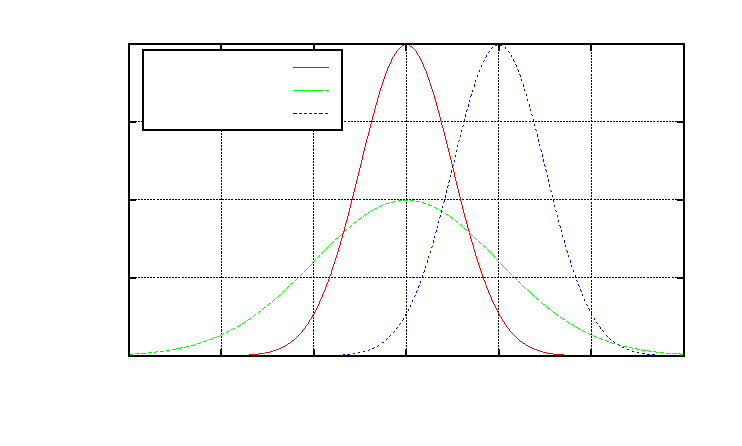
\includegraphics{normal_dist}}%
    \gplfronttext
  \end{picture}%
\endgroup

\caption{Täthetsfunktioner till normalfördelningar med olika värden på
väntevärdet $\mu$ och standardavvikelsen $\sigma$. Varje kurva har den
klassiska Gau\ss{}iska klockformen.}\label{fig:normal_dist}
\end{figure}

Kvadraten i exponentialen ger täthetsfunktionen den
klassiska klockformen hos en Gau\ss{}isk kurva, och faktorn framför
säkerställer att den totala integralen
\begin{equation}
\int_{-\infty}^{\infty} f(x)\id{x} = 1.
\end{equation}
Detta är något som \emph{gäller för alla täthetsfunktioner}. 


Normalfördelningen kallas just ''normal'' för att det finns en sats
som säger att i princip alla slumpfenomen blir normalfördelade om
samma process upprepas väldigt många gånger. Ett exempel på detta är
om man sannolikheten att få ett visst antal ''klave'' efter flera
slantsinglingar. Den här egenskapen gör att de allra flesta 
\emph{mätfelen antas vara normalfördelade}.

Vidare är normalfördelningen en väldigt trevlig fördelning att arbeta
med. Regeln för normalfördelningar är att om $X$ och $Y$ båda är
normalfördelade med väntevärde $\mu_X$ och standardavvikelse
$\sigma_X$ respektive $\mu_Y$ och $\sigma_Y$, så är 
\begin{equation}
Z=\alpha X + \beta Y
\end{equation}
också normalfördelad med väntevärde $(\alpha\mu_X+\beta\mu_Y)$ och
standardavvikelse $\sqrt{\alpha\sigma_X^2 + \beta\sigma_Y^2}$. 
Med andra ord funkar väntevärdena som man kan tro och
standardavvikelserna fungerar lite som Pythagoras sats. 


\subsection{Väntevärden, standradavvikelser och hur man skattar dem}








\section{Feluppskattningar}\label{sec:feluppskattningar}
När man vill uppskatta hur stora experimentella fel/osäkerheter man
har finns det två typer av fel och två typer av feluppskattningar. De
två typerna av fel som finns är systematiska och statistiska. Sedan är
de två typerna av feluppskattningar som man behöver kunna dels direkt
feluppskattning (av statistiska fel), dels propagering av osäkerhet. 


\subsection{Systematiska fel -- noggrannhet och precision}
\begin{figure}
\centering
\input{figurer/precision_noggrannhet.pdf_t}
\caption{Illustration av skillnaden mellan noggrannhet och
  precision. Måltavlorna representerar en mätning, där mitten på
  måltavlan svarar mot det ''sanna'' värdet. Fallen med låg
  noggrannhet svarar mot systematiska fel som inte går att avhjälpa
  med medelvärden av fler mätningar.}
\label{fig:prec_nog}
\end{figure}

Ett systematiskt fel är något som gör att ens mätresultat hela tiden
är lite fel åt något håll\footnotemark{}. Dessa karakteriseras av att
det inte hälper med flera mätningar för att få bättre mätresultat.

\footnotetext{Det behöver inet nödvändigtvis vara så att det är just
  fel åt samma håll hela tiden, men oftast är ett systematiskt fel
  något som ger en förskjutning av ens mätresultat.}

Man brukar skilja på två olika typer av godhet i mätningar. Det finns
dels noggrannhet, dels precision. Noggrannhet, eller rikighet som det
ibland kallas, svarar mot hur nära det ''sanna'' värdet mätningarna
kommer i medel. Prescisionen svarar å andra sida mot hur tätt
mätresultaten hamnar, eller hur liten spridning man får i dem. De två
koncepten illustreras i \figref{fig:prec_nog}.  

Som kan ses i \figref{fig:prec_nog} svarar låg noggrannhet mot ett
systematiskt fel som gör att medelvärdet avviker från det ''sanna''
värdet. Vidare kan man med statistisk analys bara ta reda på
spridningen i resultaten -- alltså hur bra precision man
har. Tillsammans ger detta en ganska prekär situation att hantera i
felanalys: 
\emph{Man vill veta hur {\bf noggranna} ens mätningar är, men man kan bara
  ta reda på hur {\bf precisa} de är.} 

Sättet man löser detta på är att låtsas som att det regnar och strunta
i eventuella systematiska fel när man redovisar sin felanalys. Detta
förutsätter såklart att man verkligen har försökt eliminera alla
systematiska fel; de som är kvar är dock de som man inte kände till,
vilket betder att det i princip är omöjligt att kunna uppskatta
storleken på dem. I praktiken redovisar man oftast bara spridingen i
mätresultaten och säger att märosäkerheten är samma som spridningen. 

\subsubsection{Hanterbara systematiska fel}



\subsection{Statistiska osäkerheter och hur man uppskattar dem}
För att ta reda på precisionen i mätresultaten behövs statistik. Om
ens noggrannhet är hög, övre halvan i \figref{fig:prec_nog}, behöver
man ändå veta hur god precision man har. Gör man bara en mätning har
man ingen möjlighet att veta hur nära det ''sanna'' resultatet man
kom. Det är där man måste börja använda lite statistik. 

Säg att det finns en storhet $x$ som ska mätas, men att varje mätning
har ett mätfel~$\delta{x}$. Det som mäts blir då
\begin{equation}
\hat{x}=x+\delta{x}.
\end{equation}
Utan någon mer informationom $\delta{x}$ går det inte att säga så mycket mer
från mätningen. Men som sagts tidigare antas mätfelet $\delta{x}$ vara
normalfördelat med $\mu=0$ fast med ett okänt $\sigma$. Det är oftas
$\sigma$ som man tar reda på för att ge en osäkerhetsuppskattning av
ens mätning. 

För att få fram ett värde på $x_0$ tar man ett medelvärdet av flera
mätningar. Detta ger
\begin{equation}
\bar{x}=\frac{\hat{x}_1+\hat{x}_2 + \cdots + \hat{x}_N}{N} 
= \frac{Nx+\delta{x}_1+\delta{x}_2 + \cdots + \delta{x}_N}{N}
= x + \overline{\delta{x}}.
\end{equation}
Vi utnyttjar nu att medelvärdet
$\overline{\delta{x}}\approx\mu=0$, vilket ger att $\bar{x}\approx x$.
Här syns att antagandet $\mu=0$ betydet att det inte finnsnågot
systematiskt fel som ändrar ger ett felaktigt medelvärde.




\subsection{Felpropagering}


\subsubsection{När det handlar om ett potenssamband}


%\newpage
%\bibliographystyle{ieeetr}
%\bibliography{referenser}%kräver en fil som heter 'referenser.bib'          


\end{document}


